\subsection{AlexNet}\label{resultsAlexNet}
First of all must be noted that mainly AlexNet was chiefly used here in order to test the hypotheses about balancing the data set, data augmentation and finally batch normalisation. This is due to the fact that even a simple ResNet18 achieves accuracies so high, that it becomes difficult to discern effects in for example a confusion matrix. In confusion matrices, the row number corresponds to the (index of a) class of the true label, while the column number corresponds to the (index of a) class of the predicted label. On the trace, which includes the diagonal elements, the true positives can be found. A column, excluding the element which belongs to the trace, contains the false positives. For the false negatives, one simply needs to look at a row and exclude the element which belongs to the trace of the confusion matrix. As can be seen in Fig. \ref{fig:res18-confmatrix} almost all the elements, excluding the trace, range from single-digit numbers, including many zeros, to the low double-digit numbers. This model used a simple ResNet18 implementation, using the pre-trained version provided by PyTorch. The model achieved an accuracy of about 97.57\%, with a training split size of 0.8, a learning rate of 0.01, SGD as the optimiser, batch size 64 and early stopping with patience 5 that was triggered in epoch 41. While the confusion matrix would certainly display the effects of, for example, balancing out the dataset, with such high accuracies it's difficult to assign meaning to relative changes which seem large What seems like a meaningful improvement will yield a barely changed accuracy. Furthermore, it's much harder to visualise the effect the application of a method has when almost all the predictions are correct already, so to speak. Taking these aspects into consideration, AlexNet proved to provide accuracies which, from a qualitative standpoint, seemed to be fit for visualising effects in a confusion matrix but also not too low as to provide inconclusive results to whether the network has actually learned anything. Thus, AlexNet seems an appropriate choice for evaluating the hypotheses.
\begin{figure}[h]
	\centering
	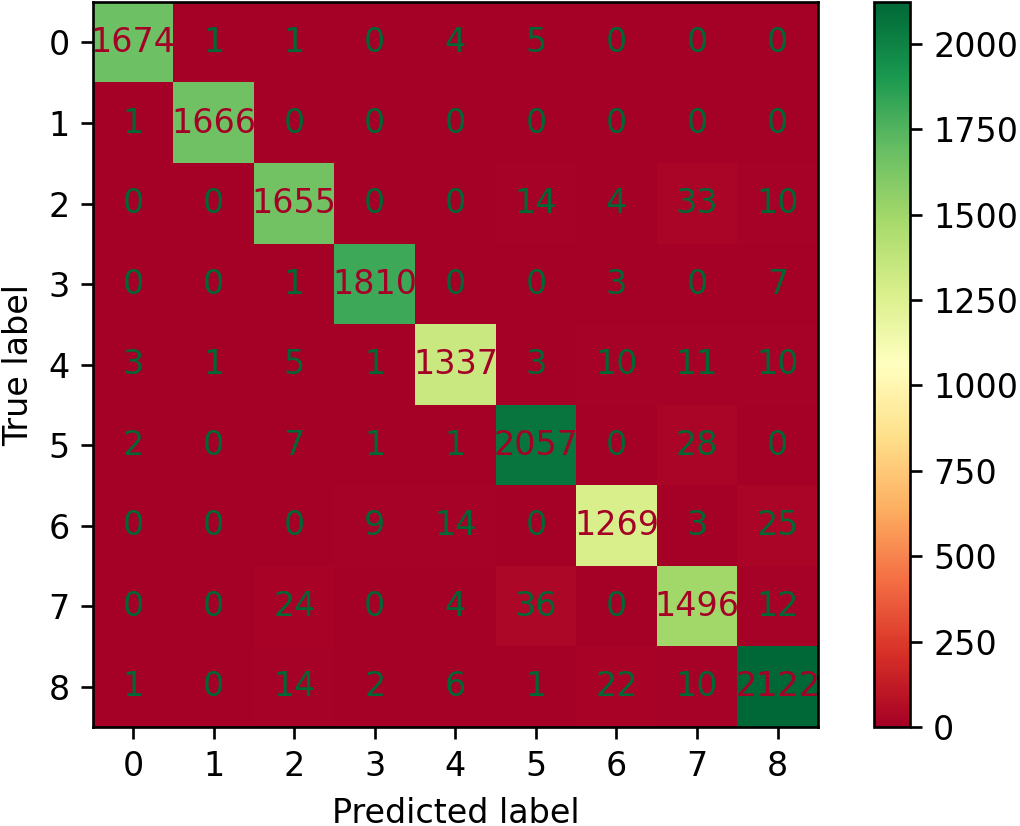
\includegraphics[scale=0.75]{./figures/model_1_no_balancing_conf_matrix_cropped.png}
	\caption{Confusion Matrix for simple ResNet 18}
	\label{fig:res18-confmatrix}
\end{figure}


\subsubsection{Experiment Balancing}\label{balancingexperiment}
Various AlexNet models were trained in order to gather evidence regarding the hypothesis that balancing of the data improves accuracy compared to a model which learned on unbalanced data. For this, the only adjustments that were made were to either enable or disable balancing and use early stopping or leave it out. All the models that were trained used a learning rate of 0.01, Adagrad as the optimiser, a split size of 0.8 and a batch size of 64. The models that didn't use early stopping were trained for 20 fixed epochs. For the early stopping version, a patience of 8 was used while a maximum number of epochs was given with 50. The results as well as the configuration for the balancing and early stopping are listed in Table \ref{balancing-table}. 
\begin{table}[h]
	\caption{AlexNet before and after balancing out the class distribution}\label{balancing-table}
	\centering
	\begin{tabular}{cccc}
		\toprule
		\multicolumn{3}{c}{} \\
		Validation Accuracy (in\%)    & Balancing     & Epochs    &Early Stopping     \\
		\midrule
		84.16    &    False    & 20    & False \\
		89.63    &    True    & 20    & False  \\
		88.94    &    False   & 44    & True \\
		91.18    &    True    & 20    & True \\
		\bottomrule
	\end{tabular}
\end{table}
Evidently, the validation accuracy improved with balancing as compared to using no balancing both for the case of early stopping not employing early stopping. For the version with the fixed number of epochs set at 20, an improvement in validation accuracy of 5.47\% was observed. In the case of employing early stopping, an improvement in validation accuracy of 2.24\% was observed. It is to be noted that for early stopping, the unbalanced version stopped after more than twice as many epochs as the balanced version while still achieving a lower validation accuracy. The confusion matrices for the models without early stopping are given in Fig. \ref{fig:balancingcombined}. A reduction in false predictions can be observed broadly across the board. It's especially noticeable for the true label 0 and the predicted label 4. Here, the false prediction shrinks by almost an entire order of magnitude from 216 to 24. Some peculiarities remain as the false predictions for true label 2 and the predicted labels 5 and 7 remain large compared to the rest, with the false predictions for 5 barely changing from 110 to 106 and the false predictions for 7 almost halving from 383 to 212. For true class 7 and predicted classes 2 and 5 the false positives also remain large relative to the other ones. In conclusion, this experiment yields evidence supporting the initial hypothesis that balancing of the data improves accuracy as compared to a model which learned on unbalanced data. Improvement is observed to happen broadly across the board, with some outliers remaining.
\begin{figure}[h]
	\centering
	\begin{subfigure}{0.49\columnwidth}
		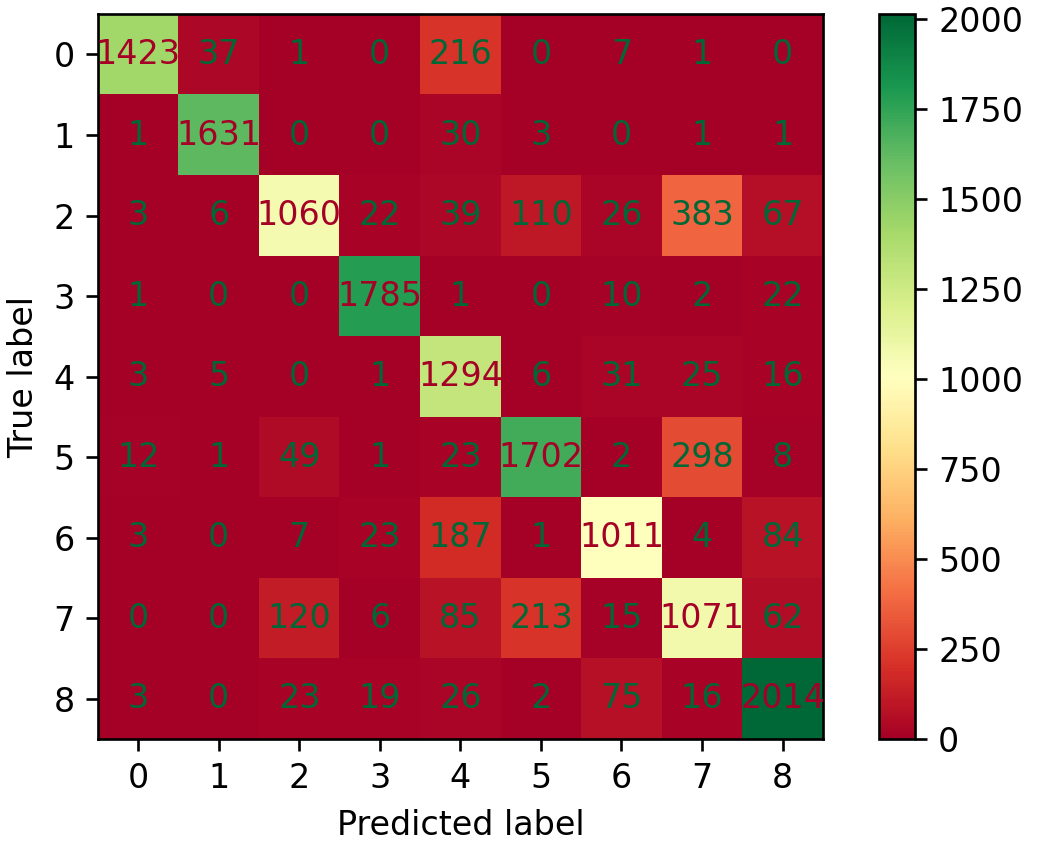
\includegraphics[width=\columnwidth]{./figures/Alex_420_no_balancing_conf_matrix_cropped.png}
		\subcaption{No Balancing}
		\label{fig:nobalancing}
	\end{subfigure} 
	~
	\begin{subfigure}{0.49\columnwidth}
		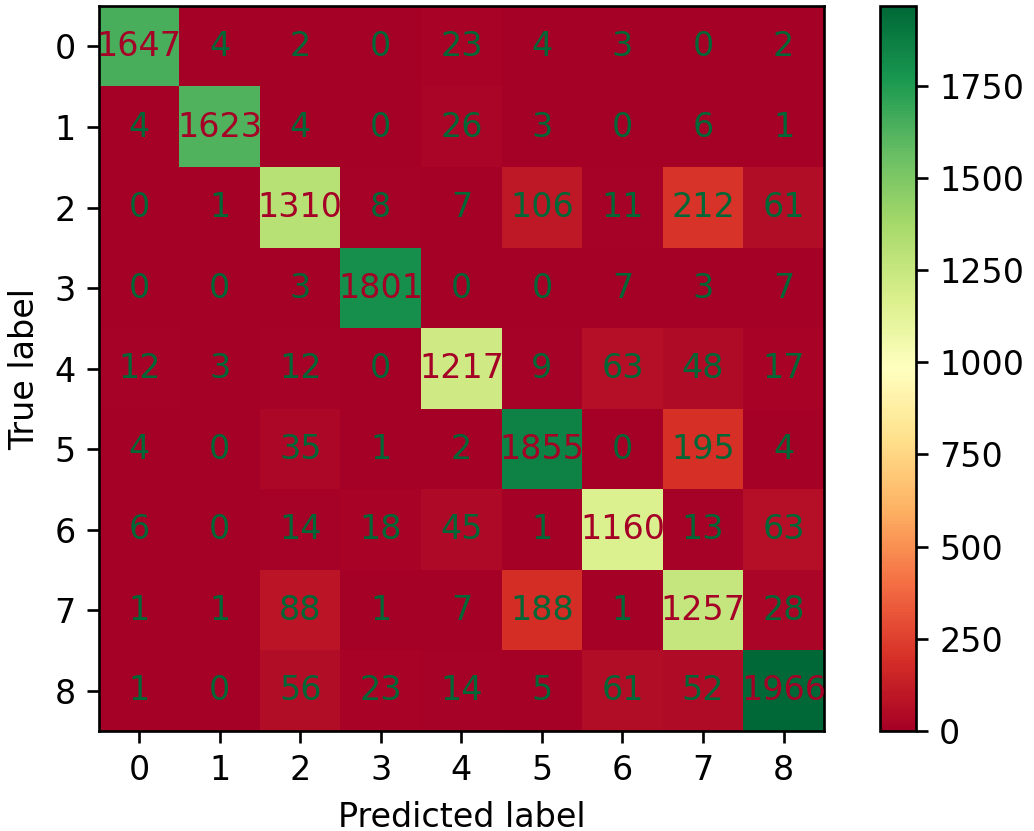
\includegraphics[width=\columnwidth]{./figures/Alex_420_with_balancing_conf_matrix_cropped.png}
		\subcaption{Balancing}
		\label{fig:balancing}
	\end{subfigure}
	\caption{Comparison confusion matrices no balancing vs balancing}
	\label{fig:balancingcombined}
\end{figure}


\subsubsection{Experiment Data Augmentation}
Going back to section \ref{augmentationtheory}, the hypothesis suggested is that data augmentation will aid with overall achieving more true positives. To test this hypothesis, several models were trained, with balancing having  been applied to all of the models. A distinction is again made between using early stopping or not. A patience of 8 has been used and a maximum number of 50 epochs for the models with early stopping. The best model is saved during training and the results are according to the best model. For the hyperparameters, the learning rate is 0.01, Adagrad is again being used as optimiser, the batch size is 64, split size 0.8. An overview over the results is given in table \ref{augmentation-table}. 
\begin{table}[h]
	\caption{AlexNet before and after augmenting the data}\label{augmentation-table}
	\centering
	\begin{tabular}{cccc}
		\toprule
		\multicolumn{3}{c}{} \\
		Validation Accuracy (in\%)     & Augmentation    &     Epochs    &Early Stopping  \\
		\midrule
		89.63    &    False    &    20    &    False  \\
		86.00   &    True    &    20    &    False  \\
		91.18    &    False    &    20    &    True  \\
		92.88    &    True    &    49    &    True  \\
		\bottomrule
	\end{tabular}
\end{table}
As can be seen, a reduction in accuracy has actually occurred when a fixed number of epochs was used. A reduction of 3.63\% occurred there. On the other hand, for the early stopping, accuracy increased by 1.7\%. However, it is to be noted that for the model with early stopping but without augmentation, coincidentally the training went on for 28 epochs with the best model being found in epoch 20, while for the model with augmentation the entire epochs were exhausted and the bets model found in epoch 49. These results do not unequivocally support or undermine the initial hypothesis.
\begin{figure}[h]
	\centering
	\begin{subfigure}{0.49\columnwidth}
		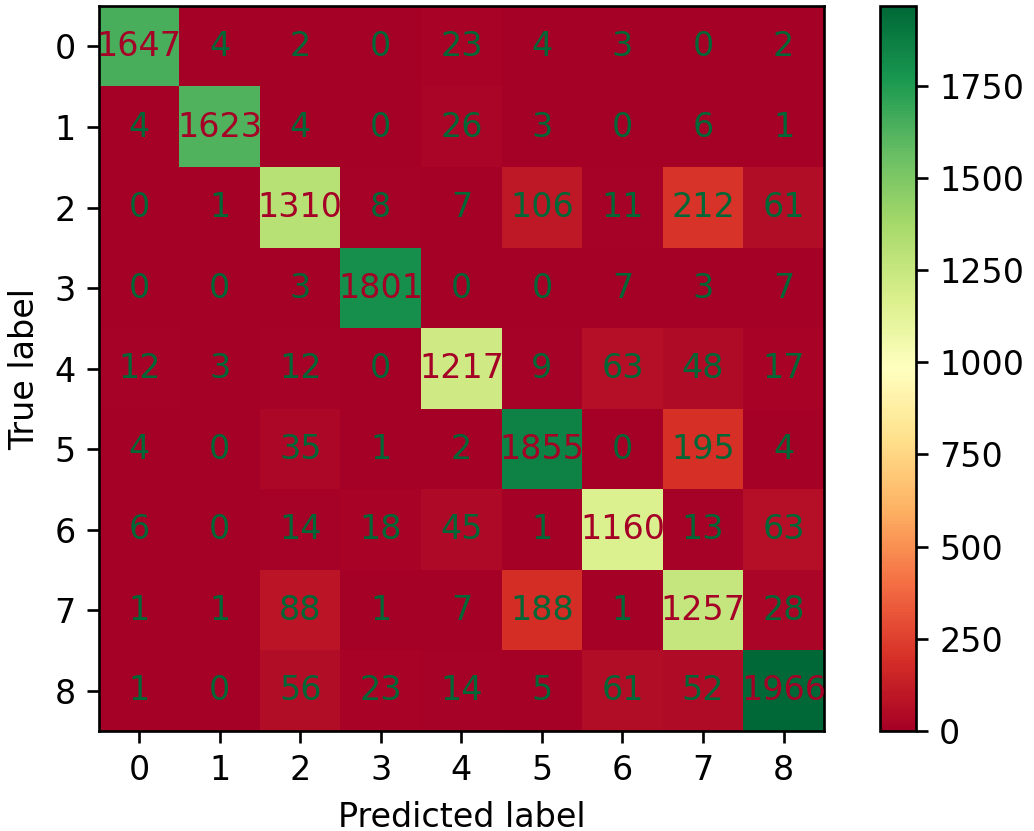
\includegraphics[width=\columnwidth]{./figures/Alex_420_with_balancing_conf_matrix_cropped.png}
		\subcaption{No Augmentation}
		\label{fig:noaugmentation}
	\end{subfigure} 
	~
	\begin{subfigure}{0.49\columnwidth}
		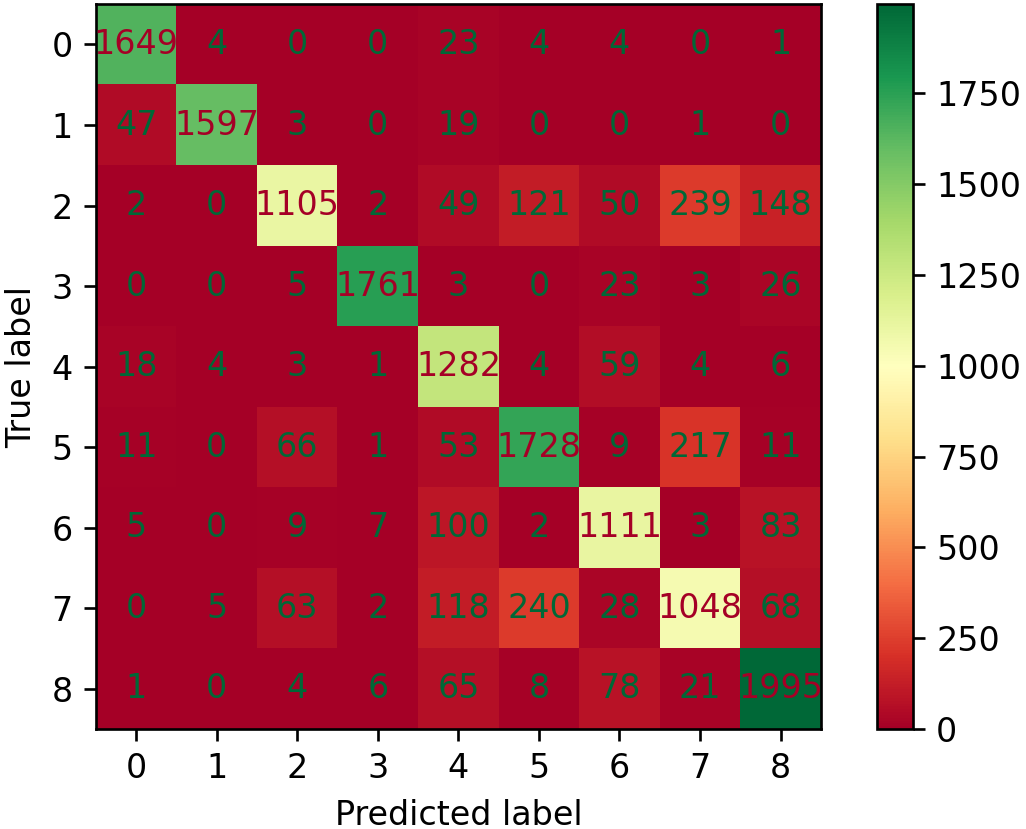
\includegraphics[width=\columnwidth]{./figures/Alex_420_augment_conf_matrix_cropped.png}
		\subcaption{Augmentation}
		\label{fig:augmentation}
	\end{subfigure}
	\caption{Comparison confusion matrices no augmentation vs augmentation}
	\label{fig:augmenetationcombined}
\end{figure}
Looking at the confusion matrix, no clear conclusion can be drawn either. From the confusion matrix without early stopping, presented in Fig. \ref{fig:augmenetationcombined}, it can be seen that the variation introduced by the data augmentation seemingly leads to drastically worse classification, for example for the true label 7 and predicted label 4. Here, without data augmentation only 7 images are incorrectly classified to be of label 4 when in reality they're label 7, but with data augmentation 118 images are incorrectly classified to be of label 4 when in reality they're label 7. That's a increase of more than 16 times, granted that the number of incorrectly classified data points there was initially just 7, a single-digit number. However, one could speculate whether the augmentation in this case lead to the model learning wrong features, thus causing a decline in validation accuracy.\newline
Taking a look at the models with early stopping, largely a broad decrease in false classified images can be observed. A suspicious rise in misclassifications is also present. Here, for the true label 5 and  predicted label 4, before augmentation 46 images were predicted and after augmentation 90, which is almost an exactly two-fold increase. This might be an indication for a wrong feature being learned but apart from this one entry, no other entry provides evidence in favour of this speculation. In conclusion it can be noted that the results for models without early stopping and with early stopping are contrary, with the former providing evidence against the initial hypothesis that data augmentation will aid with overall achieving more true positives while the latter would support such a claim.
\begin{figure}[h]
	\centering
	\begin{subfigure}{0.49\columnwidth}
		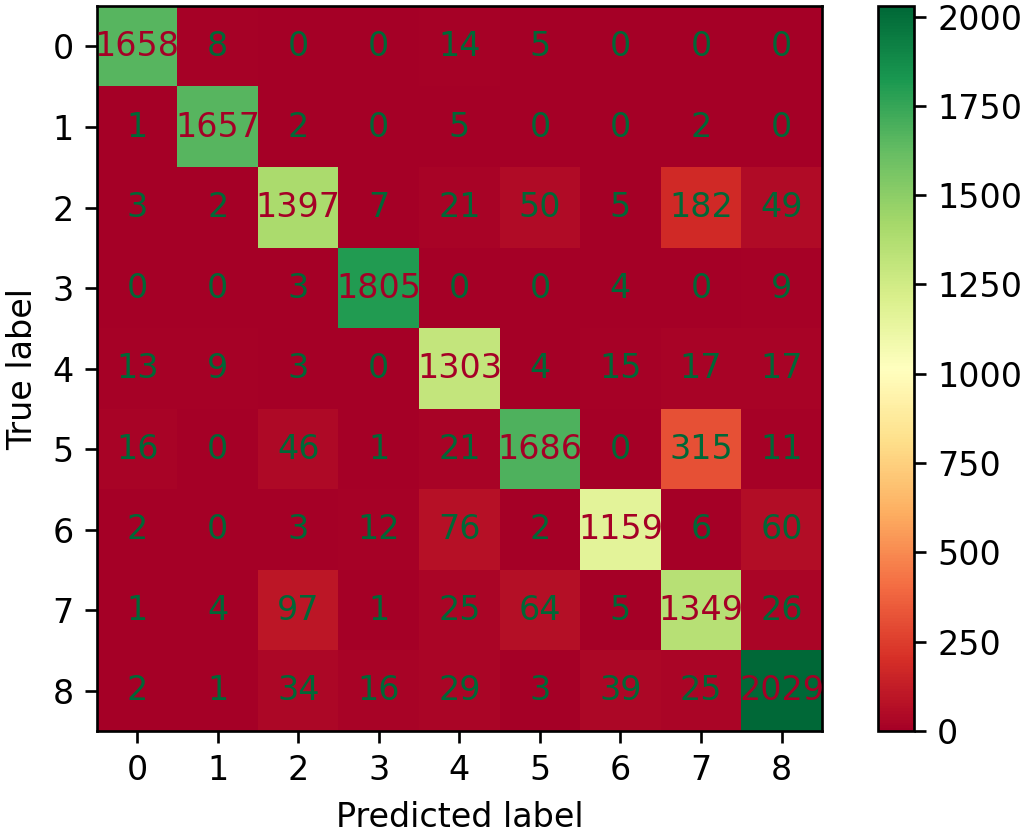
\includegraphics[width=\columnwidth]{./figures/Alex_4_with_balancing_conf_matrix_cropped.png}
		\subcaption{No Augmentation}
		\label{fig:noaugmentationearly}
	\end{subfigure} 
	~
	\begin{subfigure}{0.49\columnwidth}
		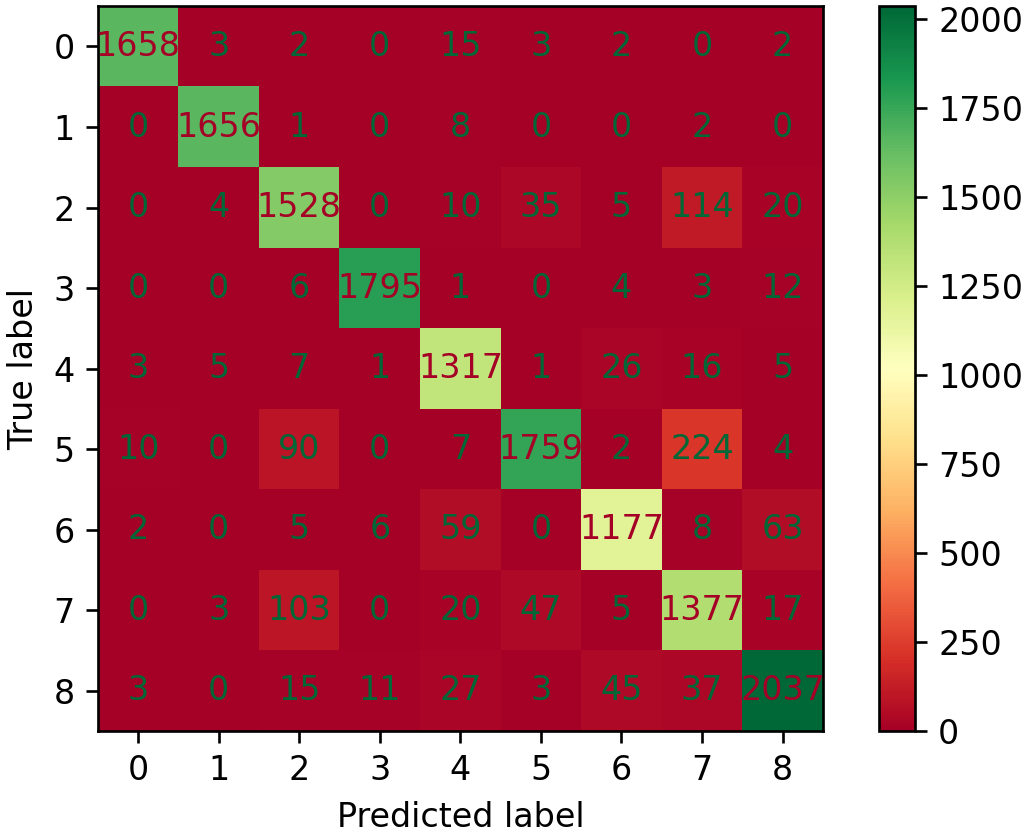
\includegraphics[width=\columnwidth]{./figures/Alex_4_with_augment_conf_matrix_cropped.png}
		\subcaption{Augmentation}
		\label{fig:augmentationearly}
	\end{subfigure}
	\caption{Comparison confusion matrices no augmentation vs augmentation with early stopping}
	\label{fig:augearlycombined}
\end{figure}



\subsubsection{Experiment Batch Normalisation}
For this experiment, the AlexNet architecture provided by PyTorch \cite{pytorchAlexNet} was modified to include batch normalisation layers after every convolution layer. The code for this is included in the appendix. Continuing from section \ref{batchnormtheory}, the hypothesis is that when training a model (in this case AlexNet) without batch normalisation layers and with batch normalisation layers, the performance across the evaluation metrics should improve ceteris paribus. To put this hypothesis to test, one AlexNet model was trained without batch normalisation layers and two models implemented to include batch normalisation layers were trained. Training was done using a learning rate of 0.001, a balanced and augmented dataset, split size of 0.8, batch size of 64, using Adagrad as the optimiser, having determined the maximum number of epochs as 150 and including early stopping with patience 8. During training, the early stopping criterion was hit for all the models 1,2,3 and the best model was found in epoch 34, 63 and 27 respectively. The results of this training can be seen in Table \ref{batchnorm-table}. While model 2 achieved an increase of validation accuracy of 0.21\% as compared to model 1, model 3 actually had a lower validation accuracy as compared to model 1, by 0.87\%. All in all, the increase or decrease doesn't exceed 1\% and also doesn't fall short of 0.1\%. Qualitatively speaking, one might call these changes to the validation accuracy small. This begs the question whether batch normalisation has really affected what the model learned here in a meaningful way. Such a change can't be made out in the validation accuracy. A possible explanation for why no such change is seen could be that AlexNet simply is not deep enough for batch normalisation to exert a big influence. Santurkar et al. describe applying batch normalisation to networks with a depth of 25 layers \citep{santurkar2018does}. AlexNet falls short of even 10 layers. In conclusion, the experiment of applying batch normalisation to the AlexNet architecture did not result in evidence supporting the intial hypothesis that batch normalisation would enhance performance.
\begin{table}[h]
	\caption{AlexNet before and after augmenting the data}\label{batchnorm-table}
	\centering
	\begin{tabular}{ccc}
		\toprule
		\multicolumn{3}{c}{} \\
		Validation Accuracy (in\%)     & Batch Normalisation    &     Model  \# \\
		\midrule
		97.29    &    False    &    1\\
		97.50   &    True    &    2\\
		96.42    &    True    &    3 \\
		\bottomrule
	\end{tabular}
\end{table}





